\chapter{Structure \ooad[71]}\label{chp:structure}
In the structure activity an extension of the problem-domain description to include structural relations between classes. Including relations between objects. The result of the structure activity is a class diagram.

\begin{figure}[H]
    \center
    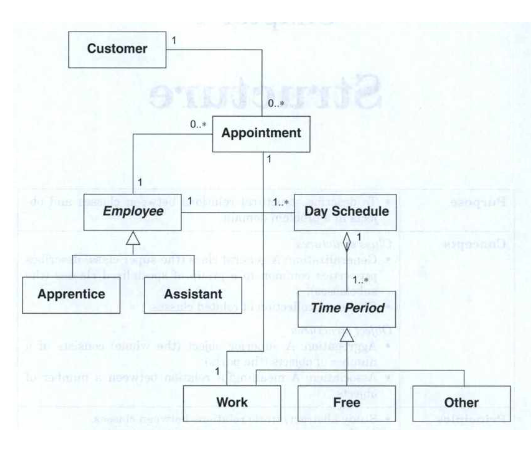
\includegraphics[width=\linewidth*3/4]{chapters/structure/figures/class_diagram.png}
    \caption{Class diagram example \ooad[72]}
    \label{fig:structure_class_diagram}
\end{figure}

\section{Class Structure}
Class structures express static, conceptual relations between classes. They connect classes, and the relationship doesn't change unless the description itself changes.

\subsection*{Generalization}
A general class(super-class) that describes properties common to a group of specialized classes(sub-classes). It's a relation between two or more specialized classes(sub-class) and a general class(super-class). Everything that holds true for the super-class also hold for any sub-classes. Programmingvise its inheritance/extending a super class.\\
This can be tested with "is-a", eg. "doctor is a person" etc.

\subsection*{Cluster}
A collection of related classes. Classes within a structure is usually connected by a generalization class, eg. cars like in \href{fig:structure_cluster_example}{the example below}. Alternatively connected through aggregation structure.
\begin{figure}[H]
    \center
    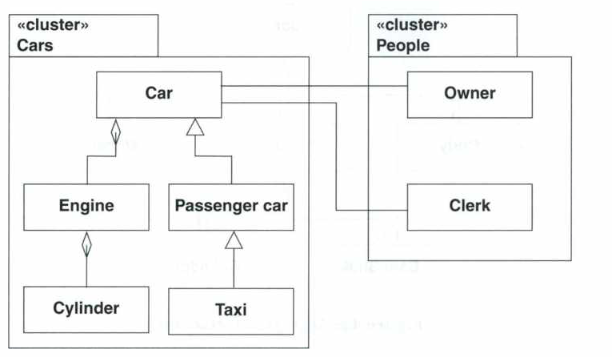
\includegraphics[width=\linewidth*3/4]{chapters/structure/figures/cluster_example.png}
    \caption{Example of clusters and cluster structure \ooad[77]}
    \label{fig:structure_cluster_example}
\end{figure}

\section{Object Structure}
Object structures express dynamic, concrete relations between objects. Theses relationship can change dynamically without changing the underlying description.

\subsection*{Aggregation}
A superior object (the whole) consists of anumber of objects (the part). It's a relation between two or more objects. It expresses that one object is a fundamental and defining part of the other.
\begin{figure}[H]
    \center
    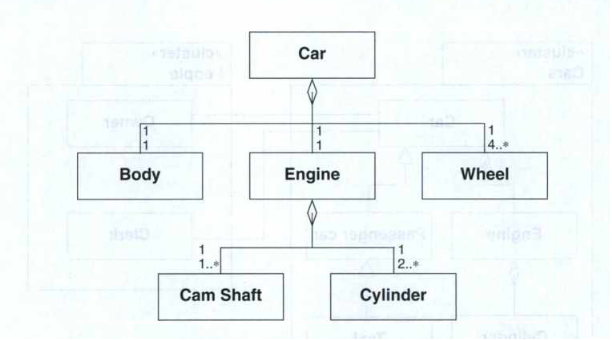
\includegraphics[width=\linewidth*3/4]{chapters/structure/figures/aggregation_structure.png}
    \caption{Aggregation structure example \ooad[78]}
    \label{fig:structure_aggregation_example}
\end{figure}
\subsection*{Association}
A meaningful relation between a number of objects. Objects are not a defining part of an object. The association structure does not define ranking

\section{The Activity}
\begin{figure}[H]
    \center
    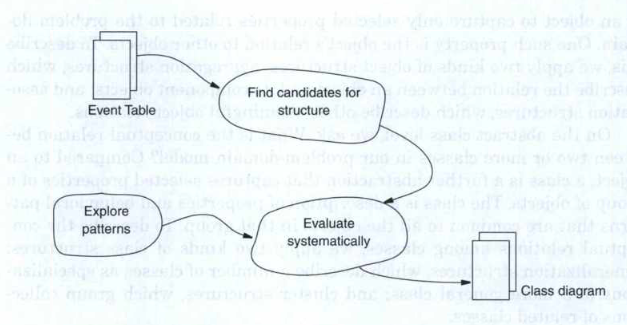
\includegraphics[width=\linewidth*3/4]{chapters/structure/figures/structure_activity.png}
    \caption{Sub-activities involved in the structure activity \ooad[74]}
    \label{fig:structure_structure_activity}
\end{figure}

\section{Finding Structure \ooad[79]}
\subsection*{Finding Candidates}
Similarly to selecting classes and events, it all starts with selecting candidates by brainstorming or other means.

\subsubsection*{Identify Generalization \ooad[80]}
Do this by taking all classes and pair them to see if one is a generalization of the other. \\
Then determine whether it's a relevant relation.\\
Then try to create a relevant specialized or generalized class.

\subsubsection*{Identify Aggregation \ooad[80]}
Find classes with objects that has a decomposition\footnote{Decomposit: The combining of distinct parts or elements to form a whole} object of the other classes. The whole is considered to be superior to its parts, as is reflected in the class diagram by the vertical placement.\\ 
Determine if it's relevant to aggregate the objects of a selected class into a new one. \\
Our third approach is to determine if each class can be decomposed few relevant classes that do not yet exist in the model. Alternatively, consider aggregating the objects of a selected class into a new class.
\\\\
Softer definitions of aggregation:
\begin{itemize}
    \item Whole-part, in which the whole is the sum of the parts, if adding or removing any part, the whole fundamental changes.
    \item Container-Content, in which the whole is a container for the parts, if adding or removing any content, the fundamental properties of the whole doesn't change.
    \item Union-Member, in which the whole is an organized union of members. It doesn't change the union fundamentally by adding or removing a few members. However, there is a lower limit on the number of members, as it is artificial to model a union without members.
\end{itemize}

\subsubsection*{Identify Associations}
See if the remaing class pairs can be meaningfully related. This is done when the relation needs to be administrated, monitored or controlled.

\subsubsection*{Identify Clusters}
Increase class diagrams clarity by organizing conceptually related classes into clusters. A class is not allowed to be in two different clusters.

\section{Explore Patterns \ooad[82]}
\subsection*{The Relation Pattern}
Used when a relation between two objects carry it's own properties.

\subsection*{The Hierarchy Pattern}
When the relation is between multiple objects and are in a hierarchy, where each level organizes into the hierachy. Eg. Student is related to a class which is related to a semester... etc.\\
A variation of this can also have objects related to multiple on a higher level. In this situation the elements are not mutually exclusive.

\subsection*{The Item-Descriptor Pattern}
Where a descriptor class defines specific properties shared by all related objects. This is important in situation where multiple copies are treated as seperate entities, but still share specific properties between them.

\section{Evaluate Systematically \ooad[86]}
\principle[Model only the neccessary structural relations]
When evaluating structural relations, it's beneficial to follow certain criteria:
\begin{itemize}
    \item Structures must be  used correctly \ooad[86].
    \item Structures must be conceptually true \ooad[87].
    \item Structures must be simple \ooad[88].
\end{itemize}